% Architecture of the final 1D CAE (width 16, z = 32), in the style of the CG course paper:
% tensors drawn as blocks (height ~ length, width ~ channels), trapezia for Linear layers,
% latent vector as a stack of cells, dashed groups for where each half runs.
\begin{tikzpicture}[
  font=\footnotesize,
  >={Stealth[length=1.8mm]},
  arr/.style={->, thick, black!70},
  lbl/.style={font=\scriptsize, text=black!75, align=center},
  dim/.style={font=\scriptsize, text=black!70, align=center},
  thumb/.style={inner sep=0pt}]

  \colorlet{encC}{blue!55!cyan}
  \colorlet{decC}{orange!85!red}
  \colorlet{latC}{green!50!black}

  % tensor block: x-centre, height, width, colour, name, dimension label
  \newcommand{\tensor}[6]{%
    \fill[#4!12, draw=#4!45, line width=0.4pt, rounded corners=1pt]
      ($(#1,0)+(-#3/2+0.14,-#2/2+0.14)$) rectangle ($(#1,0)+(#3/2+0.14,#2/2+0.14)$);
    \fill[#4!20, draw=#4!60, line width=0.4pt, rounded corners=1pt]
      ($(#1,0)+(-#3/2+0.07,-#2/2+0.07)$) rectangle ($(#1,0)+(#3/2+0.07,#2/2+0.07)$);
    \node[draw=#4!80!black, fill=#4!30, line width=0.5pt, rounded corners=1pt,
          minimum height=#2 cm, minimum width=#3 cm, inner sep=0pt] (#5) at (#1,0) {};
    \node[dim] at (#1,-1.55) {#6};}

  % trapezium for a Linear layer: x-centre, left half-height, right half-height, colour, name
  \newcommand{\linear}[5]{%
    \fill[#4!15, draw=#4, line width=0.6pt, rounded corners=1.5pt]
      ($(#1,0)+(-0.45,#2)$) -- ($(#1,0)+(0.45,#3)$) -- ($(#1,0)+(0.45,-#3)$) -- ($(#1,0)+(-0.45,-#2)$) -- cycle;
    \coordinate (#5w) at ($(#1,0)+(-0.45,0)$);
    \coordinate (#5e) at ($(#1,0)+(0.45,0)$);
    \node[lbl, text=#4!60!black, font=\tiny] at (#1,0) {Linear};}

  % ---------------- input ----------------
  \node[thumb] (in) at (0,0) {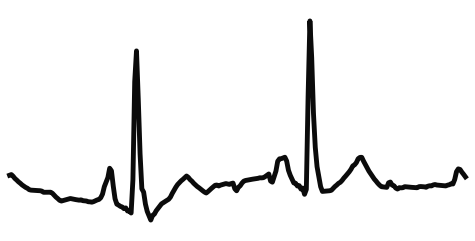
\includegraphics[width=2.3cm]{../figures/cae_in.png}};
  \node[lbl, below=1mm of in] {input \(x\)\\\(1 \times 256\) (2.56 s)};

  % ---------------- encoder ----------------
  \tensor{2.1}{2.0}{0.30}{encC}{e1}{\(16 \times 128\)}
  \tensor{3.3}{1.45}{0.50}{encC}{e2}{\(32 \times 64\)}
  \tensor{4.55}{1.0}{0.75}{encC}{e3}{\(64 \times 32\)}
  \linear{5.9}{0.75}{0.42}{encC}{le}
  \draw[arr] (in) -- (e1);
  \draw[arr] (e1) -- (e2);
  \draw[arr] (e2) -- (e3);
  \draw[arr] (e3) -- (lew);

  % ---------------- latent vector ----------------
  \begin{scope}[shift={(7.15,0)}]
    \foreach \i in {0,...,7}
      \fill[latC!18!white, draw=latC!70!black, line width=0.3pt] (-0.15,-0.72+0.18*\i) rectangle (0.15,-0.56+0.18*\i);
  \end{scope}
  \coordinate (zw) at (7.0,0); \coordinate (ze) at (7.3,0);
  \node[lbl, text=latC!60!black] at (7.15,1.0) {\(z \in \mathbb{R}^{32}\)};
  \node[dim] at (7.15,-1.55) {32};
  \draw[arr] (lee) -- (zw);

  % ---------------- link: int8 latent ----------------
  \draw[arr, latC, line width=1pt] (ze) -- node[lbl, above, text=latC!60!black] {int8, 32 B} node[lbl, below, text=latC!60!black] {BLE / Wi-Fi} (9.95,0);

  % ---------------- decoder ----------------
  \linear{10.4}{0.42}{0.75}{decC}{ld}
  \tensor{11.75}{1.0}{0.75}{decC}{d1}{\(64 \times 32\)}
  \tensor{13.05}{1.45}{0.50}{decC}{d2}{\(32 \times 64\)}
  \tensor{14.3}{2.0}{0.30}{decC}{d3}{\(16 \times 128\)}
  \tensor{15.55}{2.6}{0.30}{decC}{d4}{\(16 \times 256\)}
  \draw[arr] (lde) -- (d1);
  \draw[arr] (d1) -- (d2);
  \draw[arr] (d2) -- (d3);
  \draw[arr] (d3) -- (d4);

  % ---------------- output ----------------
  \node[thumb] (out) at (17.95,0) {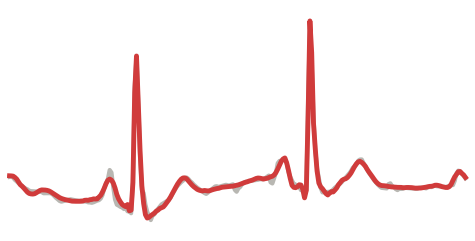
\includegraphics[width=2.3cm]{../figures/cae_out.png}};
  \node[lbl, below=1mm of out] {reconstruction \(\hat{x}\)\\\(1 \times 256\)};
  \draw[arr] (d4) -- node[lbl, above, font=\tiny] {Conv1d} (out);

  % ---------------- groups ----------------
  \draw[encC!60, dashed, rounded corners=3pt] (1.45,-2.6) rectangle (6.6,1.75);
  \node[font=\small, text=encC] (ico1) at (1.9,2.05) {\faMicrochip};
  \node[lbl, anchor=west, text=encC!60!black] at (ico1.east) {\textbf{Encoder}: ESP32-S3, 78\,560 parameters};
  \node[lbl, text=encC!60!black, font=\tiny] at (4.05,-2.15) {3 \(\times\) [Conv1d \(k{=}5\), stride 2, ReLU]\\\(\rightarrow\) Flatten \(\rightarrow\) Linear};

  \draw[decC!60, dashed, rounded corners=3pt] (9.85,-2.6) rectangle (16.1,1.75);
  \node[font=\small, text=decC] (ico2) at (10.3,2.05) {\faDesktop};
  \node[lbl, anchor=west, text=decC!60!black] at (ico2.east) {\textbf{Decoder}: PC, 81\,809 parameters};
  \node[lbl, text=decC!60!black, font=\tiny] at (12.95,-2.15) {Linear \(\rightarrow\) 3 \(\times\) [Upsample \(\times 2\),\\Conv1d \(k{=}5\), ReLU] \(\rightarrow\) Conv1d};
\end{tikzpicture}
